\documentclass[12pt,a4paper]{article}
\usepackage{amsmath}
\usepackage{amssymb}
\usepackage[brazilian]{babel}
\usepackage[utf8]{inputenc}
%\usepackage{mathtools}
\usepackage{amsthm}
\usepackage[a4paper,top=3cm,bottom=2.5cm,left=2.5cm,right=2.5cm]{geometry}
\usepackage{amstext}
\usepackage{enumitem}
\usepackage{etoolbox}
\usepackage{float}
\usepackage{hyperref}
\hypersetup{
    colorlinks=true,
    linkcolor=blue,
    filecolor=magenta,      
    urlcolor=blue_color,
}
\usepackage[ruled,vlined]{algorithm2e}
\usepackage{caption}
\usepackage{graphicx}
\captionsetup[table]{name=Tabela}
\captionsetup[figure]{name=Figura}
\usepackage{multirow}
\usepackage{multicol}
\usepackage{xcolor}
\definecolor{blue_color}{HTML}{0c71f7}

\theoremstyle{definition}
\newtheorem{teo}{Theorem}%[subsection]
\newtheorem{lema}[teo]{Lemma}
\newtheorem{prop}[teo]{Proposition}
\newtheorem{corol}[teo]{Corollary}
\newtheorem{defi}[teo]{Definition}
\newtheorem{obs}[teo]{Remark}
\newtheorem{exem}[teo]{Example}
\newtheorem{app}[teo]{Application}
\newtheorem{cond}[teo]{Condition}
\newtheorem{exe}{Exercise}

\newtheoremstyle{theoremdd}% name of the style to be used
{}% measure of space to leave above the theorem. E.g.: 3pt
{}% measure of space to leave below the theorem. E.g.: 3pt
{}% name of font to use in the body of the theorem
{}% measure of space to indent
{\itshape}% name of head font
{}% punctuation between head and body
{ }% space after theorem head; " " = normal interword space
{\thmname{#1}\thmnumber{ #2'}\thmnote{ (#3)}.}

\theoremstyle{theoremdd}

\newtheorem*{sol}{Solution}
\AtEndEnvironment{sol}{\qed}

%\DeclarePairedDelimiter\abs{\lvert}{\rvert}
\newcommand{\abs}[1]{\left\lvert#1\right\rvert}
\newcommand{\norm}[1]{\left\|#1\right\|}
\newcommand{\pint}[1]{\left\langle#1\right\rangle}
\newcommand{\ceil}[1]{\left\lceil#1\right\rceil}
\newcommand{\floor}[1]{\left\lfloor#1\right\rfloor}
\newcommand{\til}[1]{\widetilde{#1}}
\newcommand{\proj}[1]{{\rm proj}_{#1}}
\newcommand{\nat}{\mathbb{N}}
\newcommand{\real}{\mathbb{R}}
\newcommand{\inte}{\mathbb{Z}}
\newcommand{\rac}{\mathbb{Q}}
\newcommand{\comp}{\mathbb{C}}
\newcommand{\dis}{\displaystyle}
\newcommand{\de}{\partial}
\newcommand{\p}{\varphi}
\newcommand{\E}{\varepsilon}
\newcommand{\A}{\alpha}
\newcommand{\D}{\delta}
\newcommand{\T}{\mathcal{T}}
\newcommand{\im}{\mathrm{Im}\ }
\newcommand{\Int}{\mathrm{Int}\ }
\newcommand{\tr}{\mathrm{tr}\ }
\newcommand{\spann}[1]{\mathrm{span}\left\langle#1\right\rangle}
\newcommand{\vol}{\mathrm{vol}.\ }
\renewcommand\qedsymbol{$\blacksquare$}

\makeatletter
\def\subtitle#1{\gdef\@subtitle{#1}}% mudar caso queira ambiente diferente
\def\email#1{\gdef\@email{#1}}
\def\@subtitle{\@latex@warning@no@line{Hey you, no \noexpand\class given}}
\def\@maketitle{%
  \newpage \null  \vskip 2em%
  \begin{flushleft}%
  \let\footnote\thanks
    %\vskip 1.5em%
    {\large  %\lineskip .5em%
      %\begin{tabular}[t]{r@{}}%
          
     %\end{tabular}\par 
      %\begin{tabular}[t]{r@{}}%
      %{\sffamily \@class}   
     %\end{tabular}\par 
  \par}%
    %\vskip .5em% 
    {\bf\scshape \@title\\\smallskip}%\hrule}% 
   {\bf\@email}\\\smallskip
   
    \bf\text{}\@author \\\smallskip
   
  \end{flushleft}%
  \begin{center}
   { \bf\@subtitle\\\smallskip}
  \end{center}
 
  \par   \vskip 1.5em}
\makeatother


\title{Problema de Classificação de Drogas}
\author{Gabriel Felipe Dalla Stella}
\email{gabrielstella28@gmail.com}
\subtitle{\ }


\setlength{\parindent}{5pt}
\setlength{\parskip}{1em}



\begin{document}
\maketitle
\section{Introdução ao Problema}
O conjunto de dados Drug Classification foi extraído do site Kaggle (\href{https://www.kaggle.com/prathamtripathi/drug-classification}{Encontrado Aqui}).

Este conjunto de dados possui os informações médicas obtidas de pacientes que utilizaram alguma dentre as drogas denominadas A, B, C, X, e Y, nomes concedidos pelo organizador do conjunto de dados.

O objetivo deste trabalho foi utilizar as variáveis preditoras para descobrir qual a droga mais provavelmente utilizada pelos pacientes e a partir deste modelo tentar responder as seguintes perguntas:
\begin{itemize}
\item O que cada droga faz nas pessoas?
\item Há diferença entre homens e mulheres no efeito das drogas?
\item A idade tem algum efeito relevante na interação com as drogas?
\item Supondo que uma pessoa com $20$ anos, pressão alta, colesterol baixo e a razão de sódio e potássio de $13,093$, qual é a droga mais provável que essa pessoa deve ter usado?
\end{itemize}


As variáveis preditoras utilizadas do \textit{dataset} são:
\begin{itemize}
\item Age: Idade do paciente
\item Sex: Gênero do paciente (M, F)
\item BP: Pressão sanguínea do paciente (Low, Normal, High)
\item Cholesterol: Concentração de colesterol (Normal, High)
\item Na\_to\_K: Razão entre a concentração de sódio e potássio do paciente.
\end{itemize}

Para realizar essa análise, a linguagem de programação utilizada foi Python, utilizando a IDE Jupyter Notebook.

\section{Pré-processamento}

Sobre as variáveis foram utilizadas as seguintes transformações:
\begin{itemize}
\item Age: MinMaxScaler()
\item Sex: OneHotEncoding(drop=``first") (Classe positiva: M)
\item BP: OneHotEncoding(drop=``first") (Classes utilizadas: Low, Normal)
\item Cholesterol: OneHotEncoding(drop=``first") (Classe positiva: Normal)
\item Na\_to\_K: MinMaxScaler()
\end{itemize}

A opção drop=``first" é utilizada para evitar problemas de colinearidade entre as variáveis, para melhorar o desempenho dos modelos treinados.

Também utilizamos as técnicas de resampling para  melhorar o precision e o recall dos modelos, visto que os dados estão desbalanceados.

\section{Análise Gráfica}

Segue o pairplot do dataset, gerado antes do balanceamento dos dados:
\begin{center}
\begin{figure}[H]
	\centering
	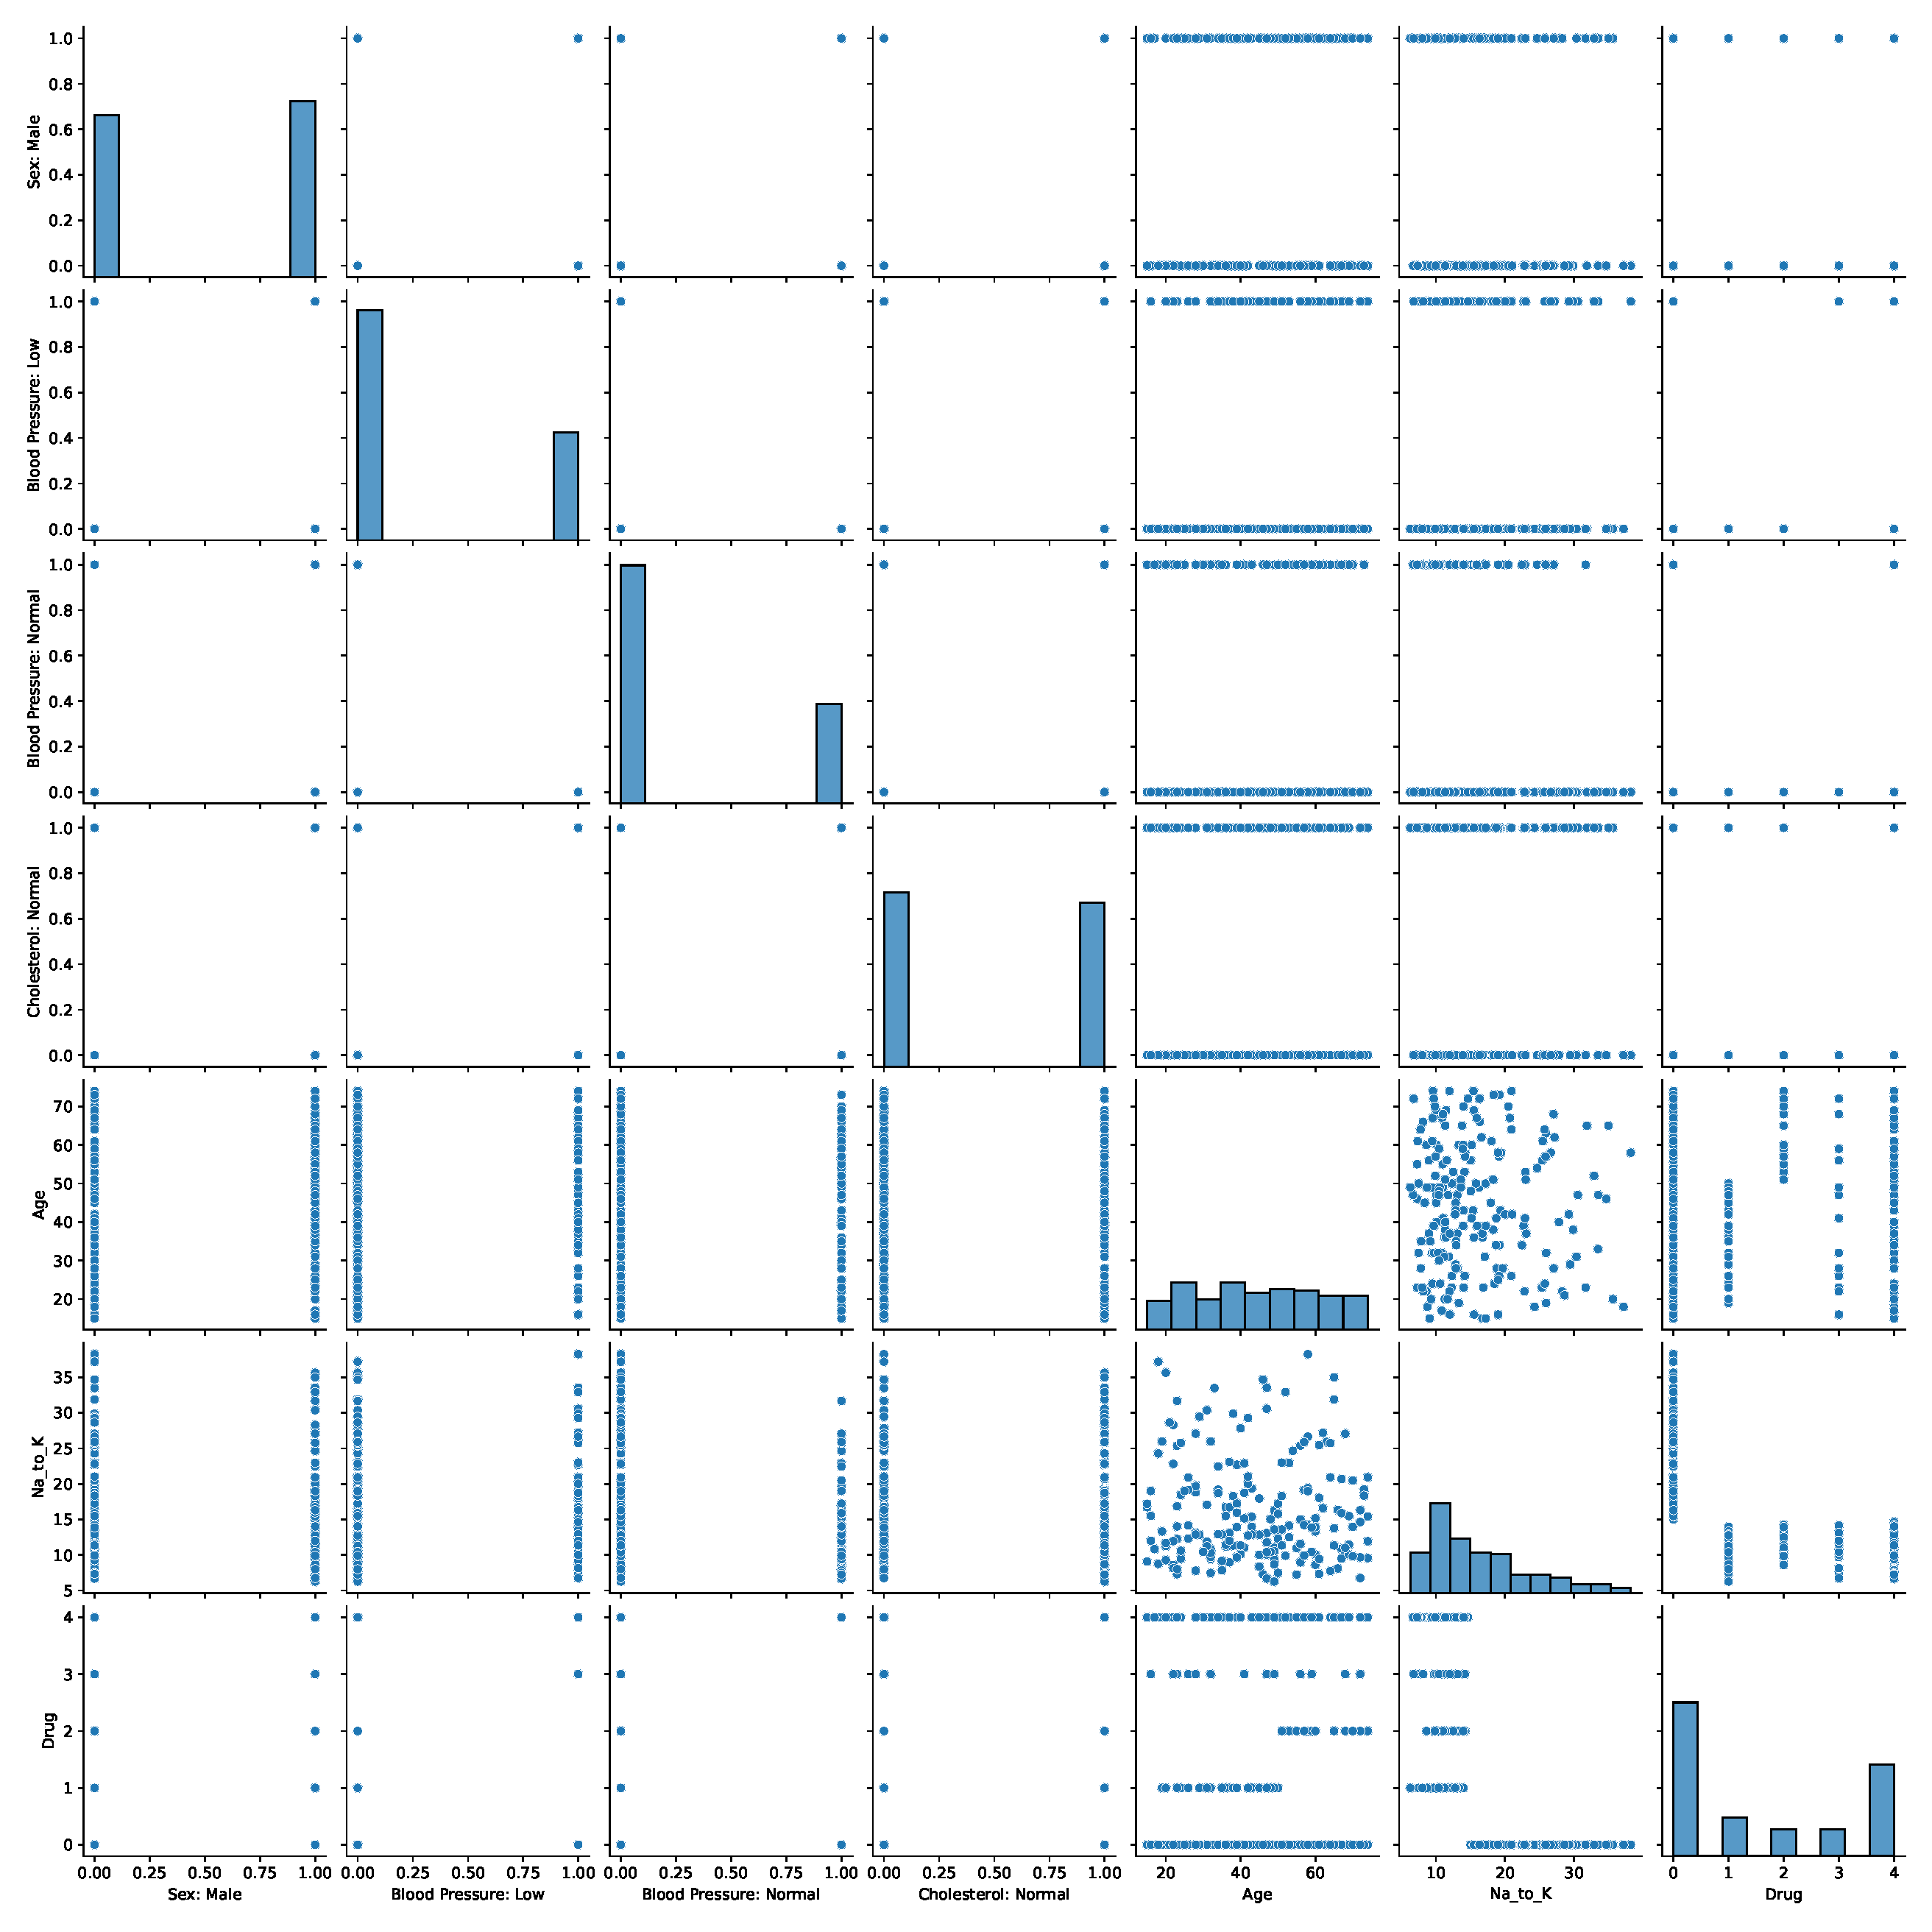
\includegraphics[height=\textwidth,width=\textwidth]{pairplot_dataset.pdf}
	\caption{Pairplot}
	\label{fig:01}
\end{figure}
\end{center}

Com a análise deste gráficos podemos gerar as seguintes hipóteses:
\begin{itemize}
\item Vemos que a concentração a razão Na\_to\_K mais alta que a mediana aparentemente indica que a droga mais provável é a que corresponde à droga Y, que corresponde ao valor 0.

\item Em geral, a droga B (valor 2) é utilizada pela população acima dos 50 anos, enquanto que a droga A (valor 1) é utilizada pela população abaixo dos 50. As drogas restantes são bem distribuídas para cada uma das idades.

\item Aparentemente a droga C (valor 3) causa um aumento no colesterol, se os pacientes, cujas informações foram coletadas, forem usuários frequentes dessa droga. Lembrando a frase clássica "Correlação não implica causalidade"

\item Quanto à pressão, as drogas A e B (valores 1 e 2) parecem ter correlação positiva com a pressão alta. A droga C (valor 3) parece estar correlacionada com a pressão baixa.
\end{itemize}

\section{Treino e Teste de modelos}

\subsection{Rede Neural}
O primeiro modelo treinado é uma rede neural profunda com as seguintes configurações:
\begin{itemize}
\item A rede é do tipo feedforward com 6 camadas escondidas.

\item Cada camada é composta por 7 neurônios, Batch Normalization e a função de ativação GELU.

\item Função de saída LogSoftmax(dim=1).

 \item A função de perda ({\it Loss Function}) é dada por NLLLoss() ({\it Negative Log-Likelihood Loss})

\item O otimizador utilizado foi o Adam com {\it learning rate} (taxa de aprendizado) de $8\mathrm{e}-5$ e {\it weight decay } (Regularização $\ell_{2}$) de $1\mathrm{e}-5$.

\item O treinamento foi realizado com {\it batch size} de 64, número de épocas $1\mathrm{e}4$ e EarlyStopping com patience 6.


\item A divisão utilizada foi de $50\%$, $25\%$ e $25\%$, para os dados de treino, validação e teste, respectivamente.
\end{itemize}

O gráfico da função de perda em cada iteração é dado por:
\begin{center}
\begin{figure}[H]
	\centering
	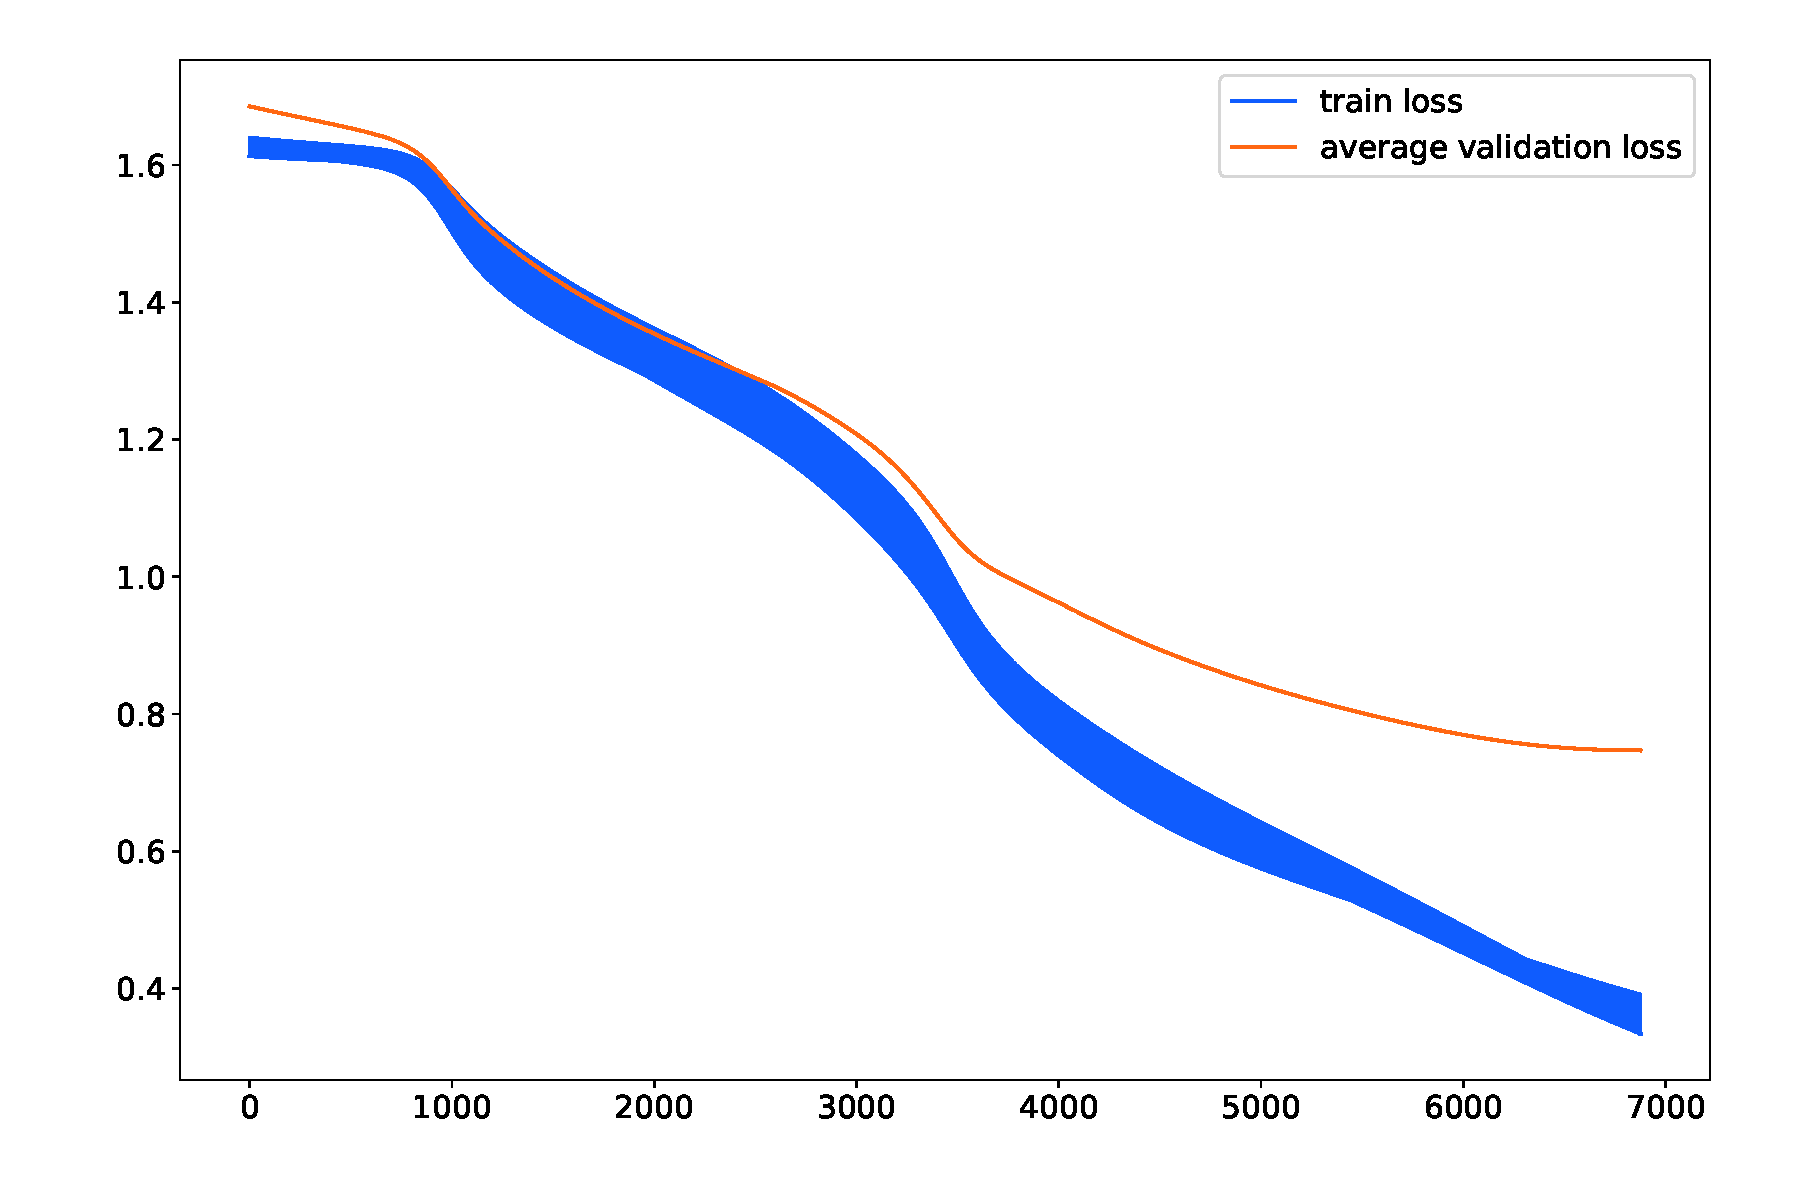
\includegraphics[height=0.667\textwidth,width=\textwidth]{Classification_NN_training_loss.pdf}
	\caption{Função perda por iteração}
	\label{fig:02}
\end{figure}
\end{center}

Nos dados de treino e validação, o desempenho foi de $88\%$ de precisão.

Verificando o desempenho do melhor classificador nos dados teste, que corresponde à um total de 50 dados, obtemos as seguintes tabelas utilizando a função classification\_report:

\begin{displaymath}
\begin{tabular}{|l|r|r|r|r|}
\hline
{} &  precision &    recall &  f1-score &  support \\
\hline
0            &   1.000000 &  0.925926 &  0.961538 &    27 \\
1            &   1.000000 &  1.000000 &  1.000000 &     2 \\
2            &   0.666667 &  1.000000 &  0.800000 &     2 \\
3            &   0.833333 &  1.000000 &  0.909091 &     5 \\
4            &   1.000000 &  1.000000 &  1.000000 &    14 \\ \hline
accuracy     &   {} &  {} &  0.960000 &     50 \\
macro avg    &   0.900000 &  0.985185 &  0.934126 &    50 \\
weighted avg &   0.970000 &  0.960000 &  0.962140 &    50 \\
\hline
\end{tabular}
\end{displaymath}
Esse classificador possui um desempenho interessante nos dados de teste. Pode ser que o número pequeno de amostras influencie a ter um alto desempenho.







\subsection{Random Forest}

O segundo modelo testado foi o Random Forest, com o método de RandomSearchCV com 20 iterações e o hiperparâmetro estimado foi o max\_depth entre 1 e 40.


Este modelo foi treinado com os mesmos dados de treino e validação da rede neural, visto que com o EarlyStopping o conjunto de validação também faz parte do treino, na rede neural. O conjunto de teste também se mantém inalterado.

A melhor performance é dada por max\_depth de 34, com desempenho de $99\%$ de precisão.


Verificando o desempenho do melhor classificador nos dados teste, que corresponde à um total de 50 dados, obtemos as seguintes tabelas utilizando a função classification\_report:

\begin{displaymath}
\begin{tabular}{|l|r|r|r|r|}
\hline
{} &  precision &  recall &  F$_{1}$-score &  support \\
\hline
0.0          &        1.0 &     1.0 &       1.0 &     27 \\
1.0          &        1.0 &     1.0 &       1.0 &      2 \\
2.0          &        1.0 &     1.0 &       1.0 &      2 \\
3.0          &        1.0 &     1.0 &       1.0 &      5 \\
4.0          &        1.0 &     1.0 &       1.0 &     14 \\ \hline
accuracy     &        {} &     {} &       1.0 &      50 \\
macro avg    &        1.0 &     1.0 &       1.0 &     50 \\
weighted avg &        1.0 &     1.0 &       1.0 &     50 \\
\hline
\end{tabular}
\end{displaymath}

Vemos um melhor desempenho nesse modelo, tanto em termos de validação, quanto em termos de dados de teste.

\section{Análise de impactos}
Para analisar os impactos de cada variável sobre as probabilidades de cada classe utilizamos a biblioteca shap.


Agora, utilizando o modelo Random Forest, que obteve um melhor desempenho, podemos realizar a inferência sobre os dados. Nesse caso podemos responder as seguintes perguntas:
\begin{itemize}
\item O que cada droga faz nas pessoas?
\item Há diferença entre homens e mulheres no efeito das drogas?
\item A idade tem algum efeito relevante na interação com as drogas?
\item Supondo que uma pessoa com $20$ anos, pressão alta, colesterol baixo e a razão de sódio e potássio de $13,093$, qual é a droga mais provável que essa pessoa deve ter usado?
\end{itemize}

\subsection{Droga Y}

A seguir temos a figura contendo as informações dos Shapley Values gerada pela biblioteca shap:
\begin{center}
\begin{figure}[H]
	\centering
	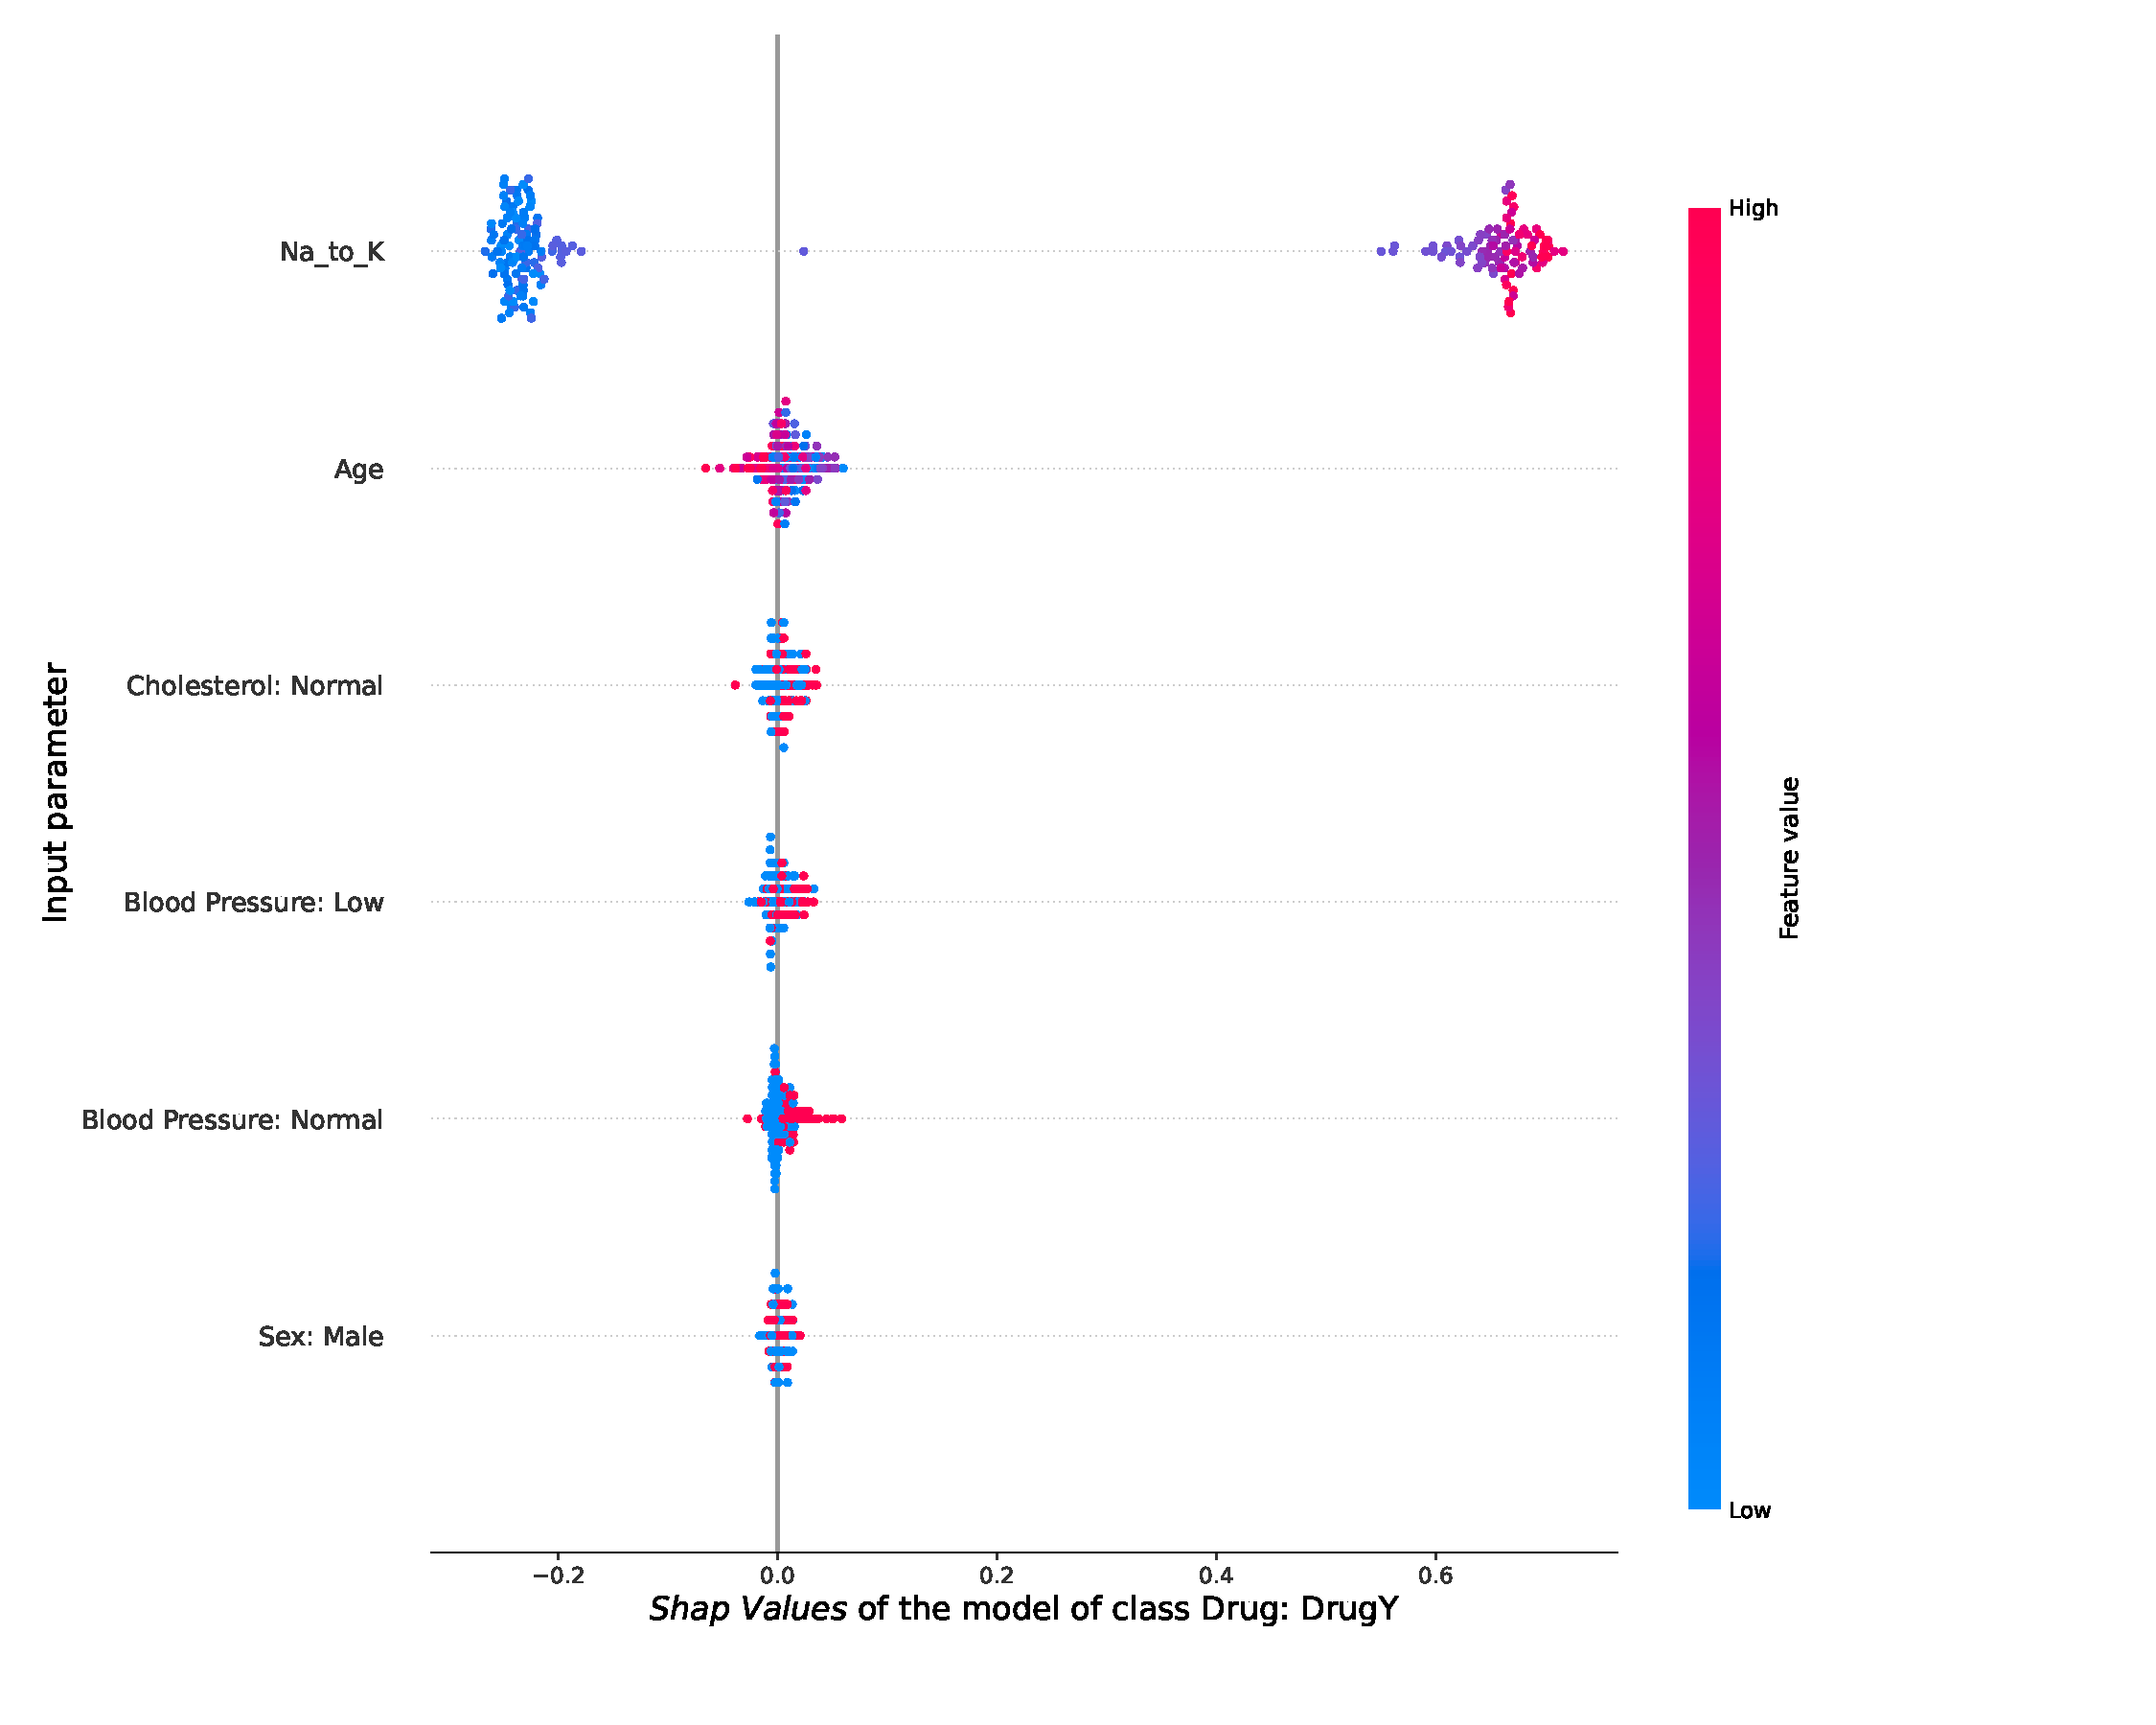
\includegraphics[scale=.40]{shap_drugY.pdf}
	\caption{Shapley Values referentes à droga Y}
	\label{fig:03}
\end{figure}
\end{center}

Para a droga Y temos as seguintes conclusões:

\begin{itemize}
\item Podemos ver que o maior impacto dessa droga é na razão entre as concentrações de sódio e potássio. Mais precisamente, quando a razão é menor, a tendência é que não seja a droga Y e para valores maiores da razão, é esperado que a droga predita seja Y.

Lembrando que essa afirmação está de acordo com a análise gráfica, onde comentamos que valores mais altos de razão Na\_to\_K tende a ser a droga Y.



\item As outras variáveis tem pouca influência sobre a predição.

\item O gênero é pouco relevante sobre a probabilidade de ser a droga Y.

\item A idade  possui pouca influência sobre a predição dessa droga.
\end{itemize}


\subsection{Droga A}
A seguir temos a figura contendo as informações dos Shapley Values gerada pela biblioteca shap:
\begin{center}
\begin{figure}[H]
	\centering
	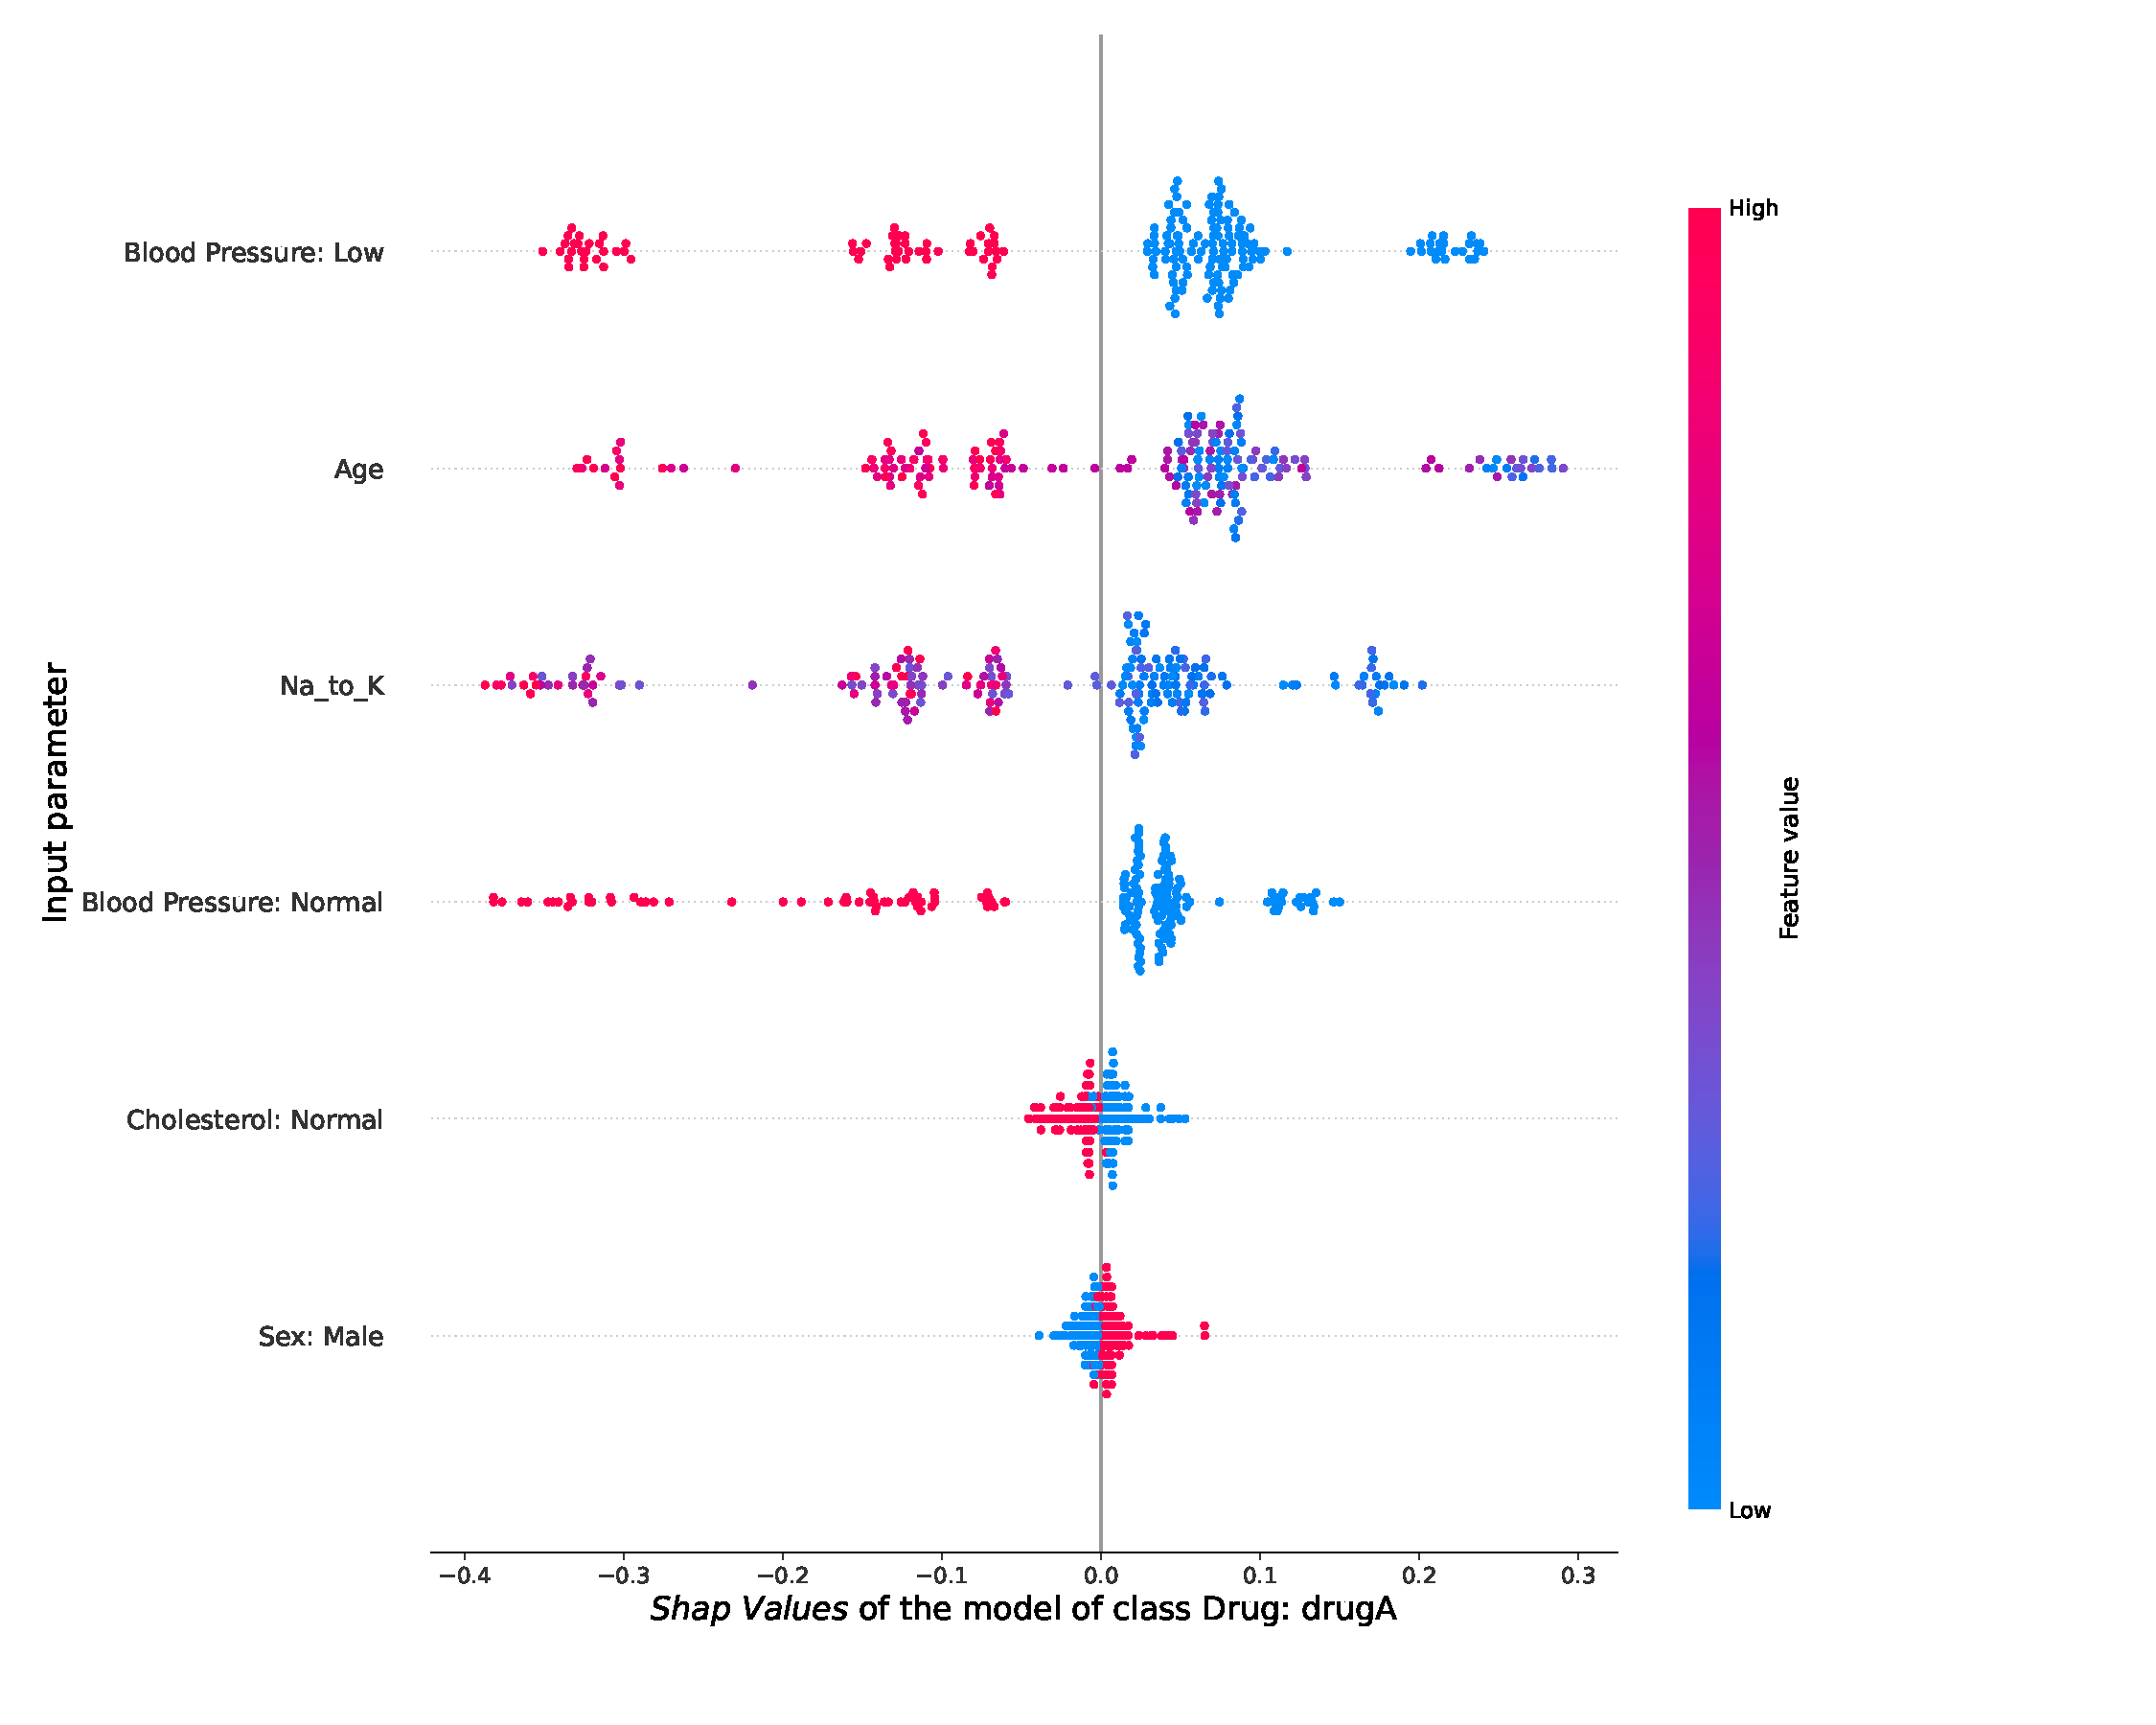
\includegraphics[scale=.40]{shap_drugA.pdf}
	\caption{Shapley Values referentes à droga A}
	\label{fig:04}
\end{figure}
\end{center}

Para a droga A temos as seguintes conclusões:

\begin{itemize}
\item Cruzando as informações de Blood Pressure: Low e Blood Pressure: Normal, vemos que pressão alta tende a aumentar a probabilidade da de ser a droga A.

Esta informação é compatível com o que foi visto na análise gráfica.

\item Valores médios a altos da razão Na\_to\_K tendem a diminuir o a probabilidade de ser a droga A.

\item Vemos que a tendência é que os mais jovens utilizem a droga A, como visto na análise gráfica.

\item A hipótese sobre o gênero é que os homens usam levemente mais essa droga que as mulheres. Porém isso deve ser melhor investigado para obter conclusões mais sólidas.

\item Outra hipótese é que o uso ou não da droga A tem leve relação positiva com o colesterol alto.
\end{itemize}


\subsection{Droga B}
A seguir temos a figura contendo as informações dos Shapley Values gerada pela biblioteca shap:
\begin{center}
\begin{figure}[H]
	\centering
	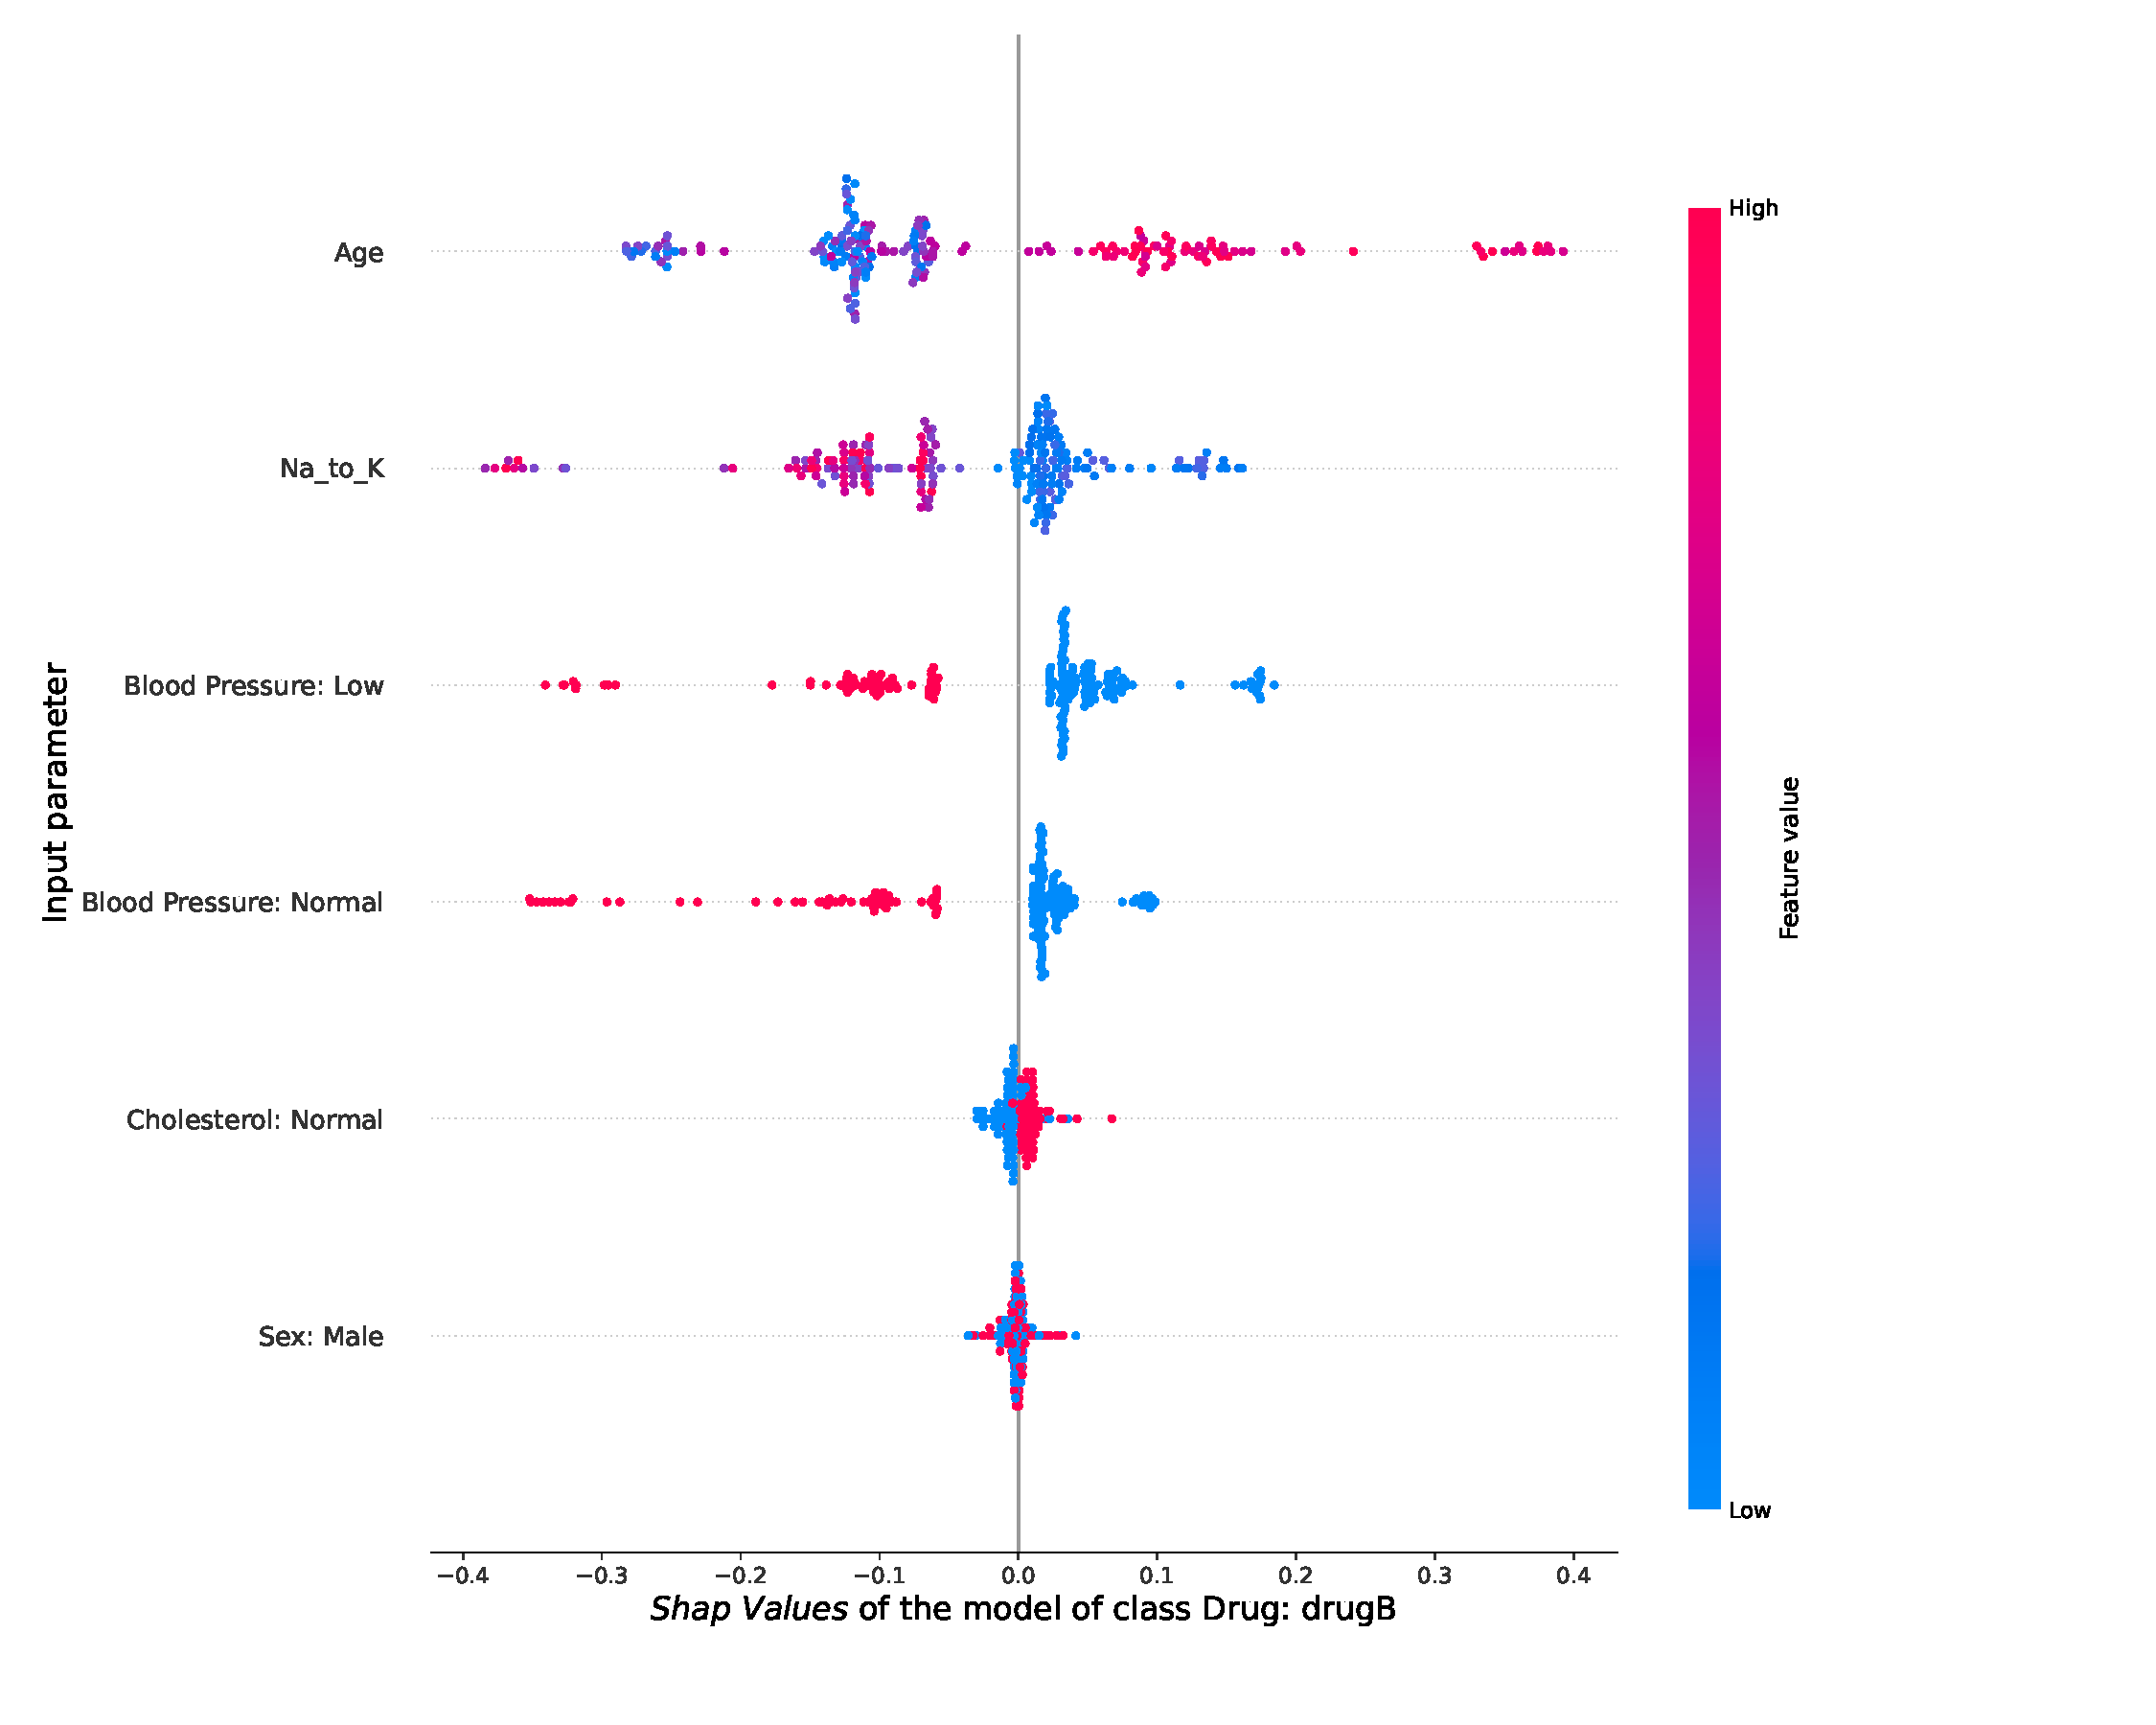
\includegraphics[scale=.40]{shap_drugB.pdf}
	\caption{Shapley Values referentes à droga B}
	\label{fig:05}
\end{figure}
\end{center}

Para a droga B temos as seguintes conclusões:

\begin{itemize}
\item Cruzando as informações de Blood Pressure: Low e Blood Pressure: Normal, vemos que pressão alta tende a aumentar a probabilidade da de ser a droga B.

Esta informação é compatível com o que foi visto na análise gráfica.

\item Valores médios a altos da razão Na\_to\_K tendem a diminuir o a probabilidade de ser a droga B.

\item Vemos que a tendência é que os mais velhos utilizem a droga B, como visto na análise gráfica.

\item Não há um gênero de preferência para o uso da droga B, mais precisamente, o gênero não nos dá informação relevante para a previsão.

\item Outra hipótese é que o uso ou não da droga A tem leve relação positiva com o colesterol normal.
\end{itemize}


\subsection{Droga C}
A seguir temos a figura contendo as informações dos Shapley Values gerada pela biblioteca shap:
\begin{center}
\begin{figure}[H]
	\centering
	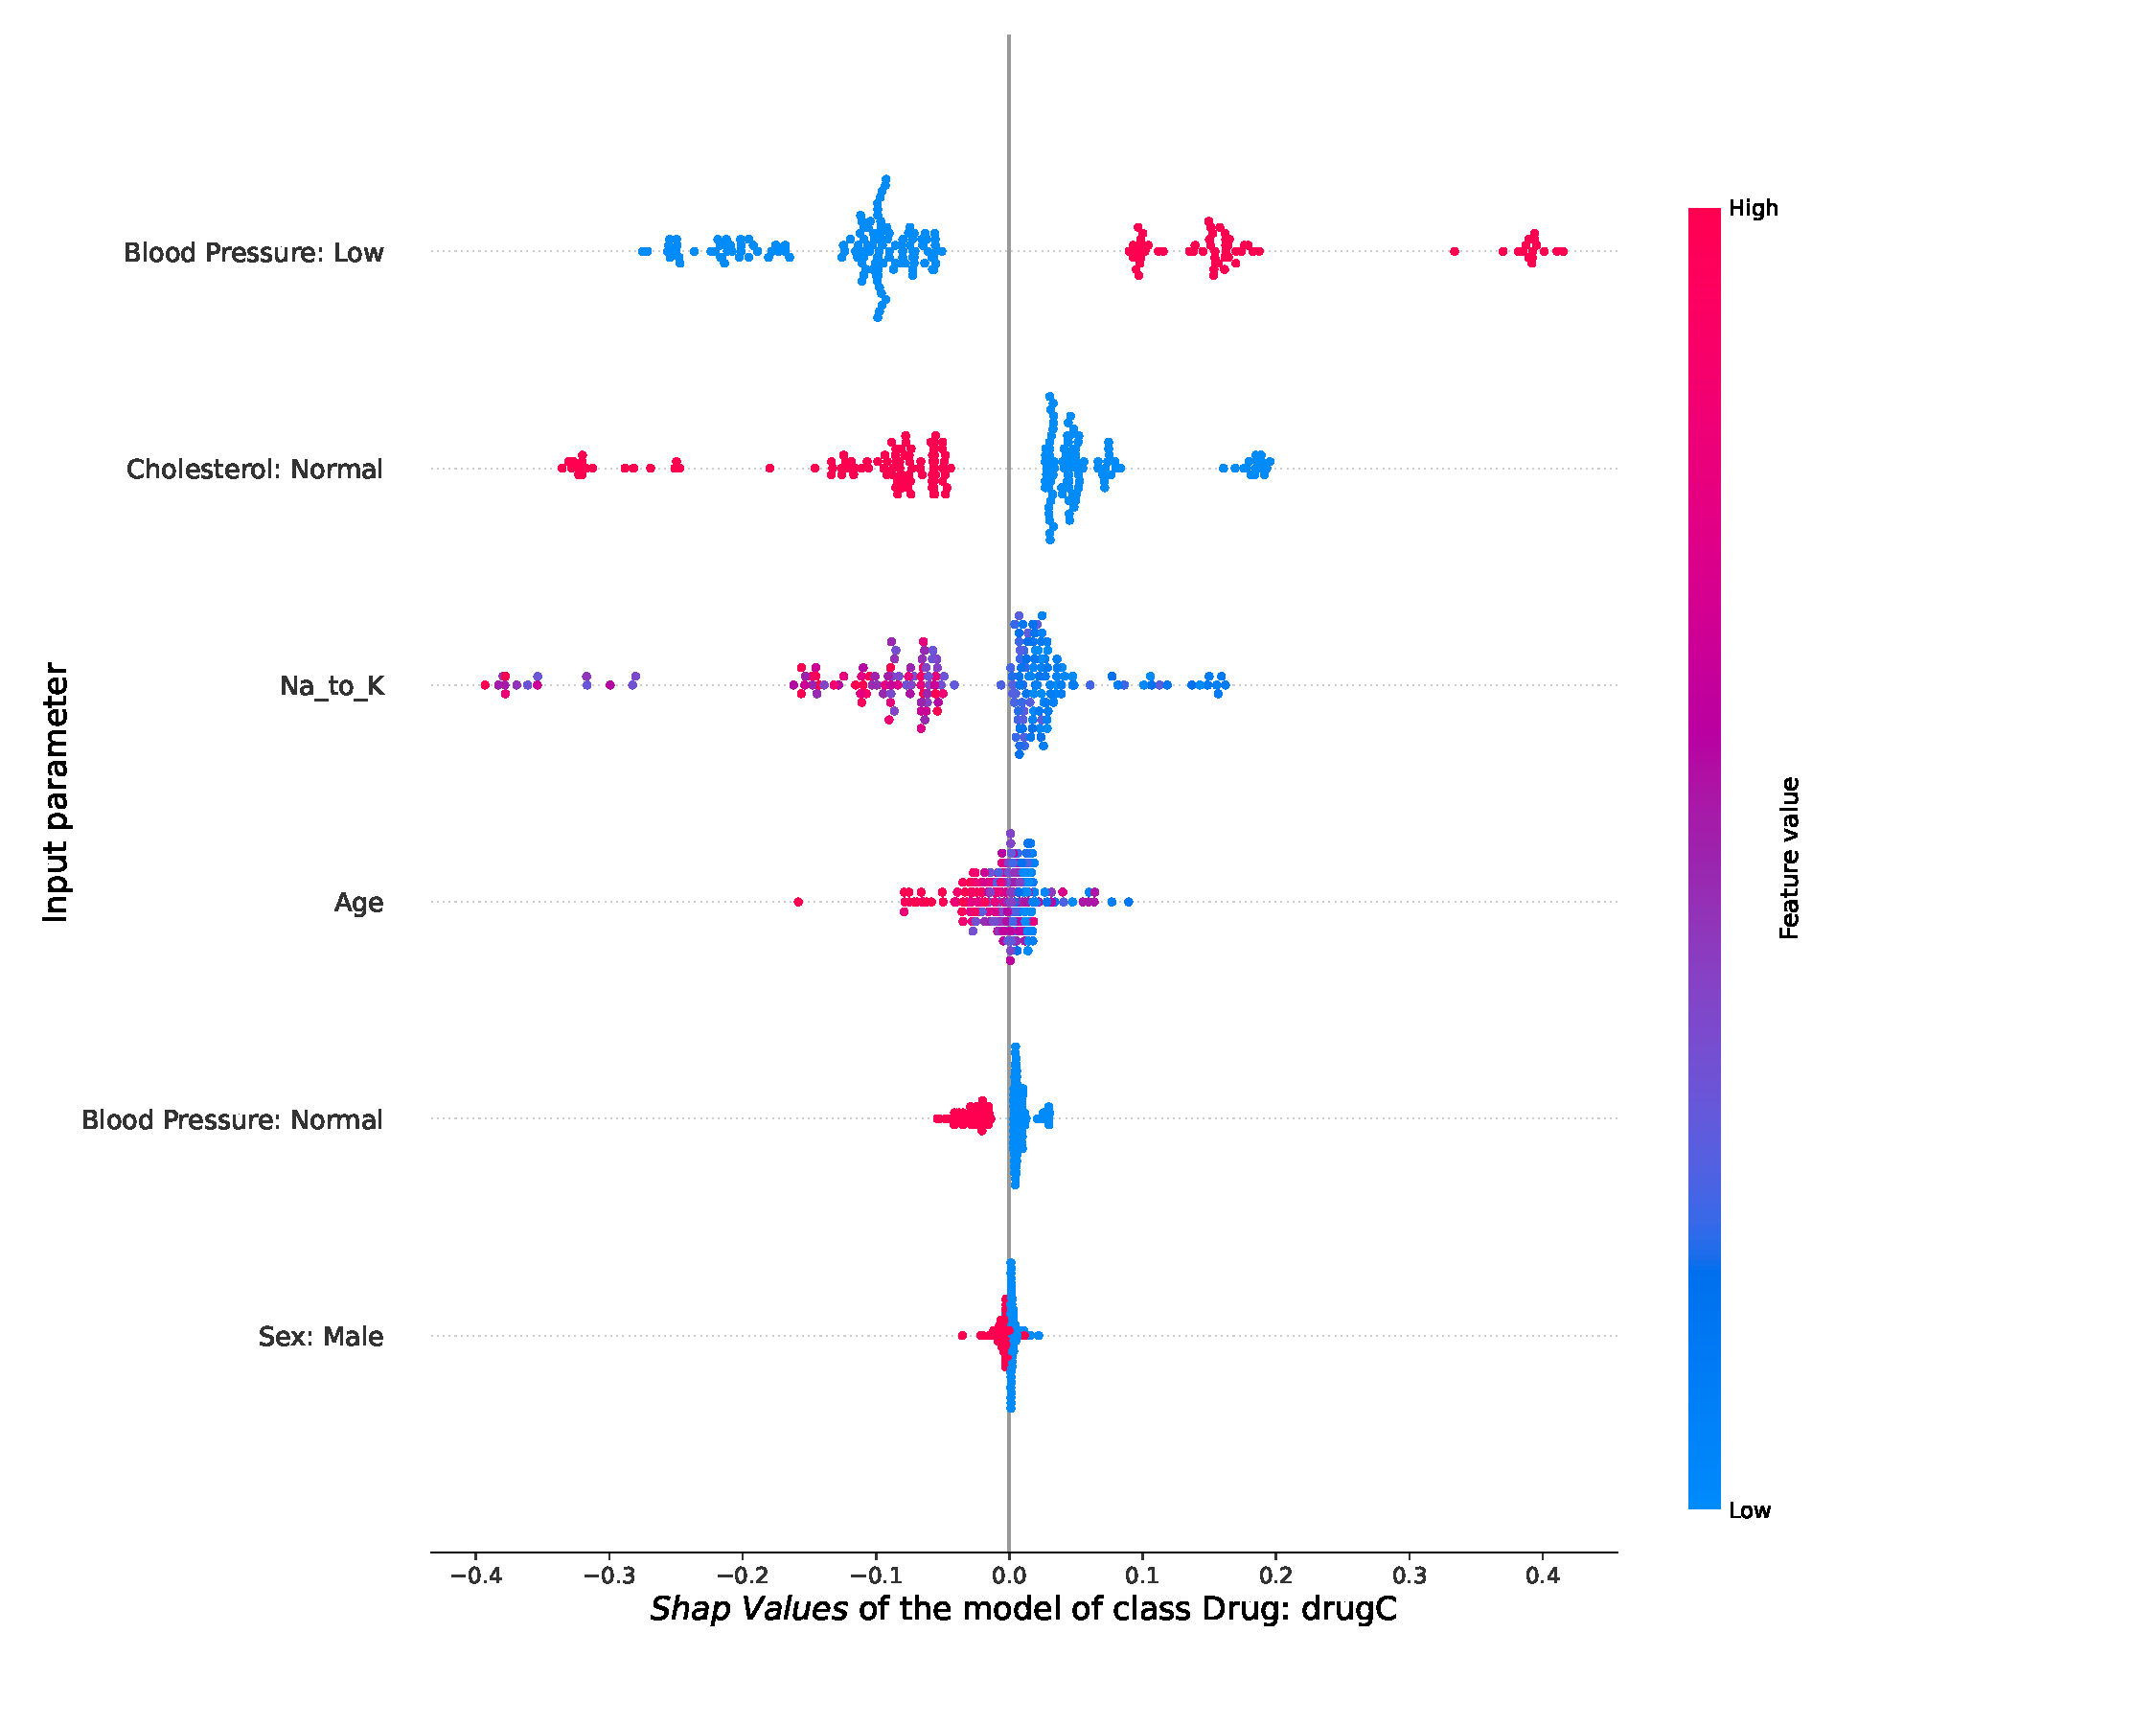
\includegraphics[scale=.40]{shap_drugC.pdf}
	\caption{Shapley Values referentes à droga C}
	\label{fig:05}
\end{figure}
\end{center}

Para a droga C temos as seguintes conclusões:

\begin{itemize}
\item Cruzando as informações de Blood Pressure: Low e Blood Pressure: Normal, vemos que pressão baixa tende a aumentar a probabilidade da de ser a droga C. Essa variável tem uma influência muito alta sobre a probabilidade.

Esta informação é compatível com o que foi visto na análise gráfica.

\item Valores médios a altos da razão Na\_to\_K tendem a diminuir o a probabilidade de ser a droga C.

\item Vemos que uma leve tendência é que os mais jovens utilizem a droga C.

\item O gênero tem influência praticamente nula sobre a probabilidade de ser a droga C.

\item Outra hipótese é que o uso ou não da droga C tem forte relação positiva com o colesterol alta.
\end{itemize}


\subsection{Droga X}
A seguir temos a figura contendo as informações dos Shapley Values gerada pela biblioteca shap:
\begin{center}
\begin{figure}[H]
	\centering
	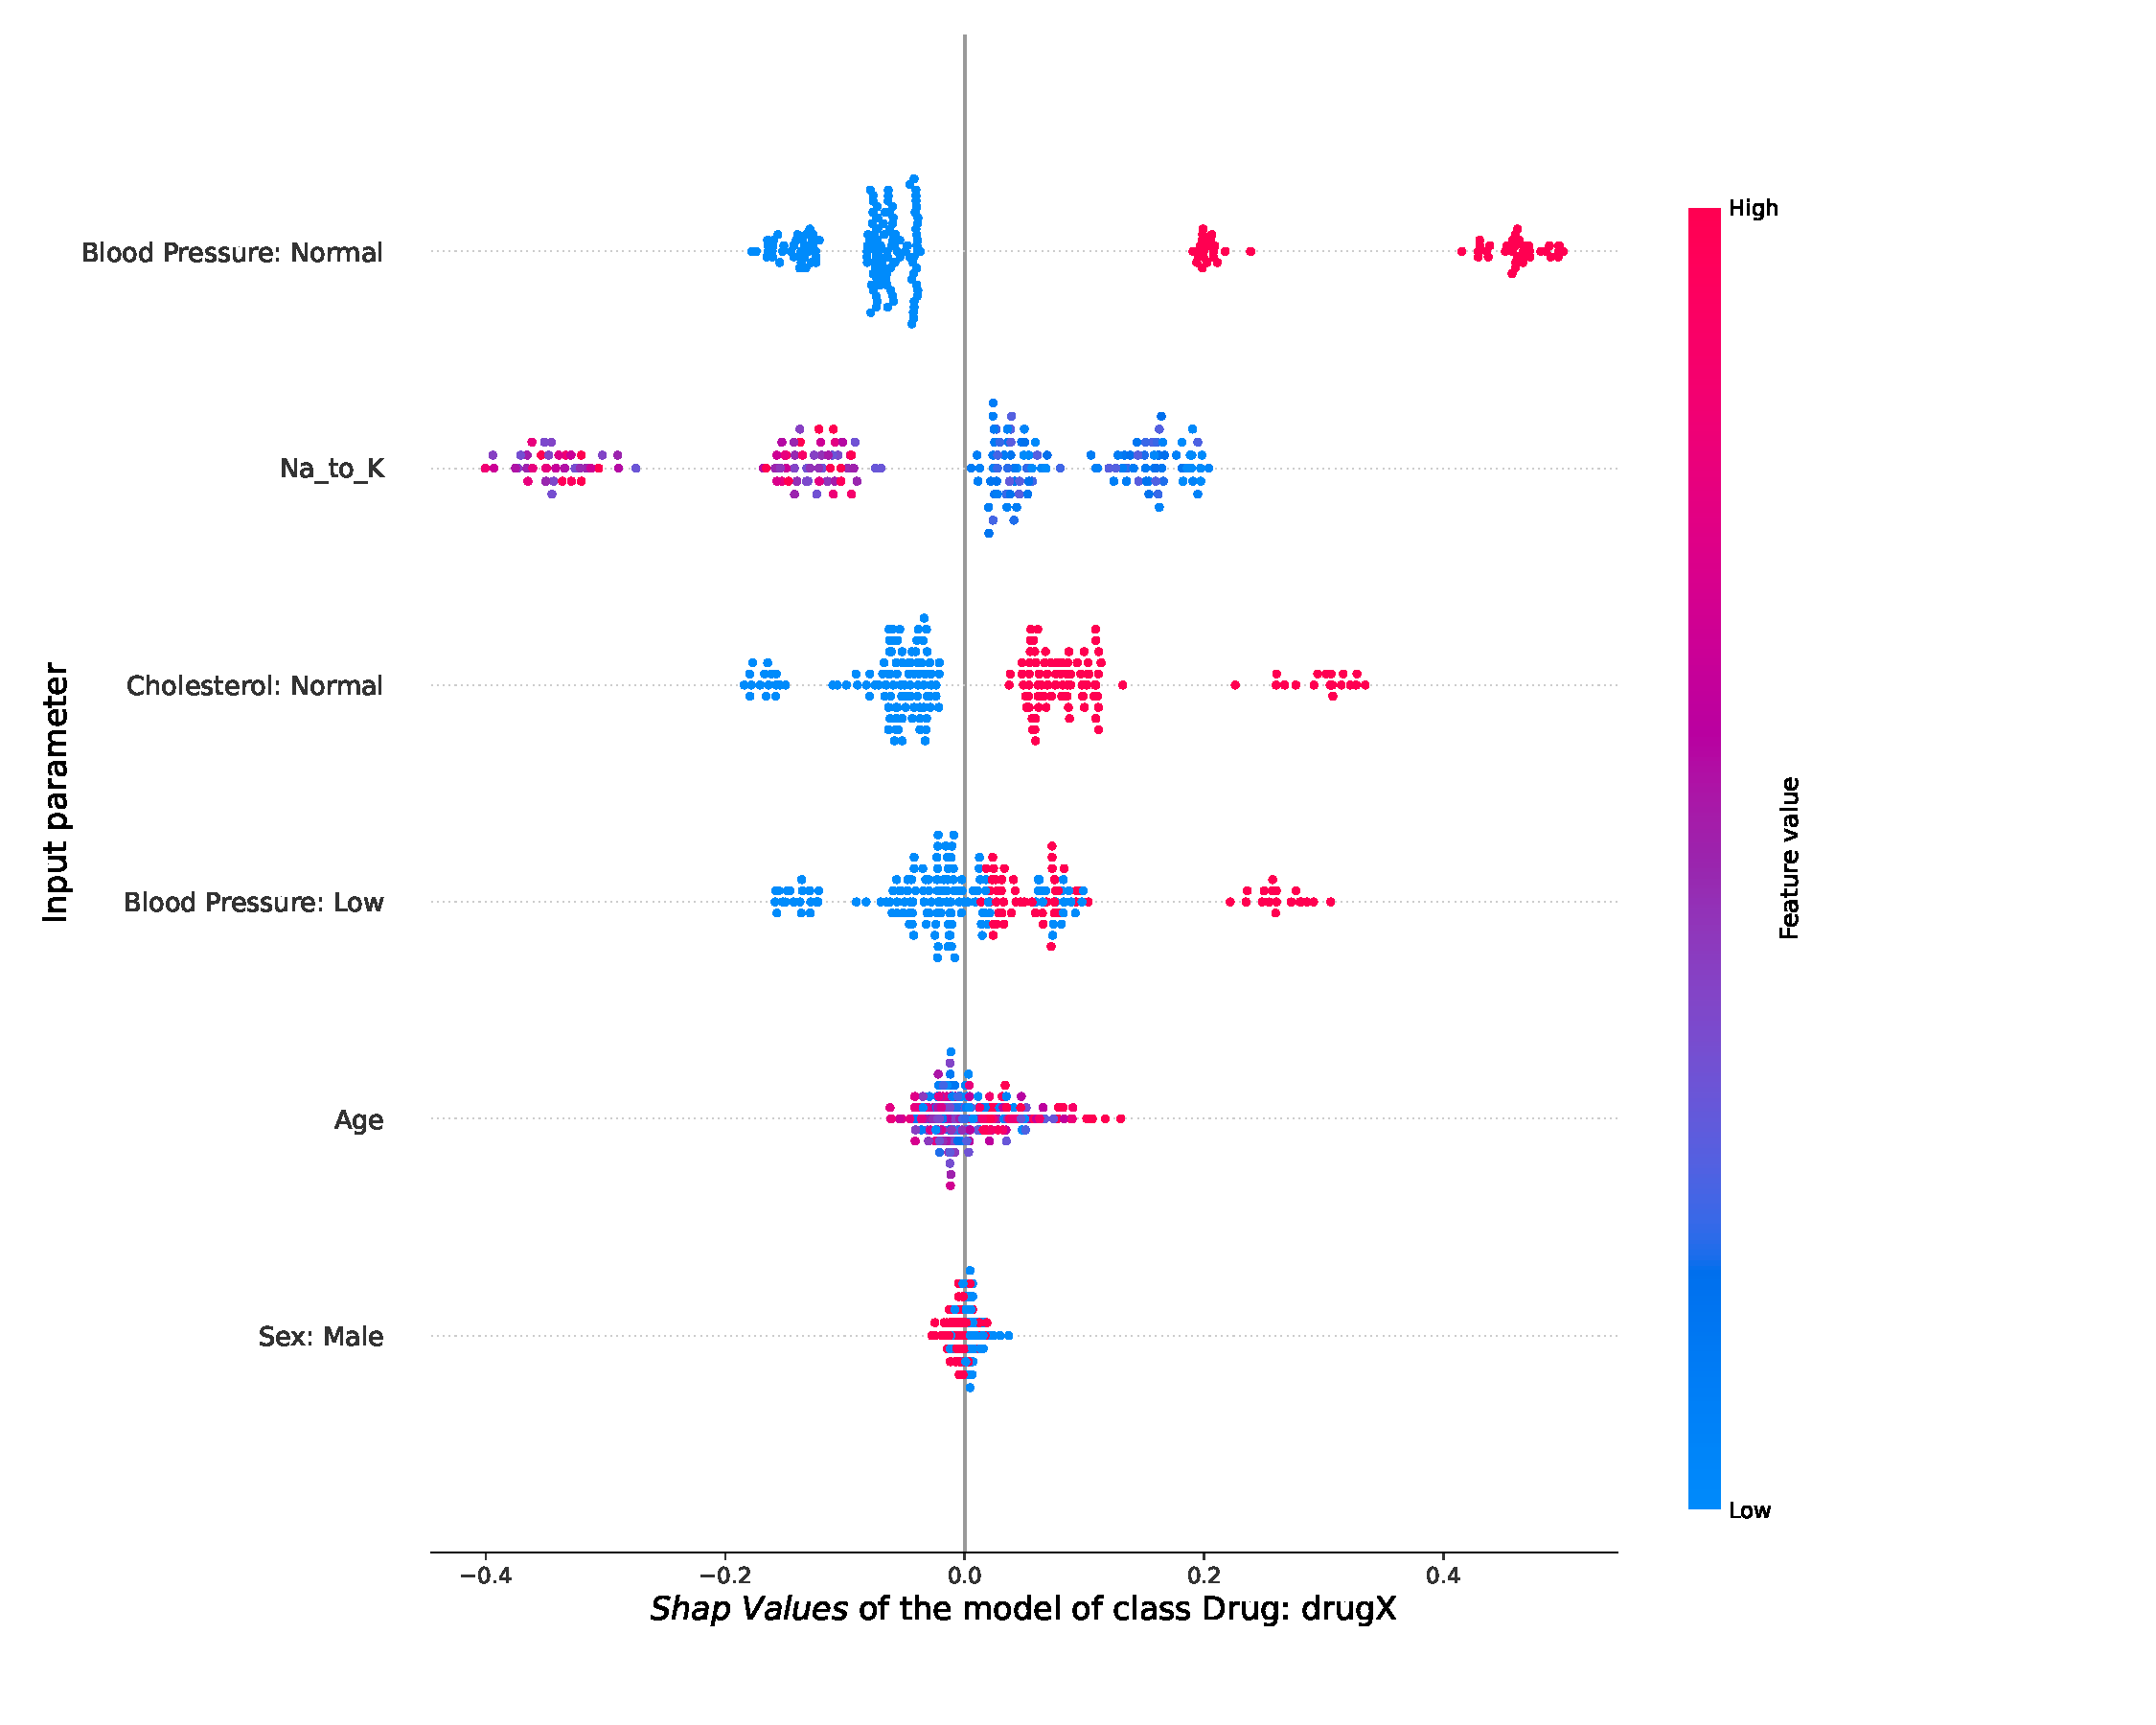
\includegraphics[scale=.40]{shap_drugX.pdf}
	\caption{Shapley Values referentes à droga X}
	\label{fig:05}
\end{figure}
\end{center}

Para a droga X temos as seguintes conclusões:

\begin{itemize}
\item Cruzando as informações de Blood Pressure: Low e Blood Pressure: Normal, vemos que os usuários da droga X tendem, em geral, a apresentar pressão baixa ou normal na coleta dos dados.

\item Valores médios a altos da razão Na\_to\_K tendem a diminuir o a probabilidade de ser a droga X.

\item A idade tem relação pouco clara com o uso da droga X.

\item O gênero tem influência praticamente nula sobre a probabilidade de ser a droga X.

\item O uso ou não da droga X tem forte relação positiva com o colesterol normal.
\end{itemize}



\end{document}
